Unsurprisingly, data collected from the GlueX detector mostly contains reaction topologies (the set of initial\-/, intermediate\-/, and final\-/state particles) which are not the channel of interest in this thesis. Additionally, due to the unavoidable finite resolution of each detector, the measured quantities such as the momentum of each particle might not exactly align with physical expectations (such as four-momentum conservation). For these reasons, we need to filter the detected data to just events which match our desired topology and kinematically fit the observables such as particle masses, decay vertices, and four-momenta with constraints that enforce conservation laws and other desirable properties.

This process begins with particle reconstruction, where the raw detector data is transformed into charged particle tracks (from the drift chambers), photon showers (from the calorimeters), and some timing data from the ST and TOF. Next, the charged tracks are matched up with their respective showers from the calorimeters, and the remaining showers are labeled as ``neutral showers'' originating from photons (or possibly large neutral particles like neutrons). At this stage, no particle identification is assigned to the charged and neutral tracks.

\subsubsection{Particle Identification Cuts}

The next stage involves filtering through reconstructed tracks to find events which match our topology. First, we apply some basic selections to the track data, including a requirement that neutral showers must have an energy of at least $\SI{100}{\mega\eV}$ and neutral showers in the BCAL must be detected in at least two detector cells. Timing cuts are then applied to whichever detector gives the best timing information (the order being BCAL, TOF, FCAL, ST). By timing, we mean the difference between the time measured in the detector and the time of the RF beam bunch measured in the TAGH/TAGM. Each set of charged tracks is identified with each charged particle in the topology (events with too many or too few charged tracks are excluded). Each hypothetical identification is then subjected to cuts on the energy lost in the drift chambers or deposited in the calorimeters. Since there are no ``missing'' final-state particles (such as a neutron) in our reaction, an additional cut is made on the missing energy (the difference between the initial energy from the beam photon and the summed energy of the final-state particles). Finally, cuts are made on the invariant mass of some particles, as well as the missing mass (squared) for the step of the reaction from which the particle originated. For example, in the reaction $\gamma p \to K_S^0 K_S^0 p \to \pi^+\pi^-\pi^+\pi^- p$, a missing mass cut applied to the recoil proton would use the difference between the (squared) invariant mass of $\gamma p$ and $4\pi p$, but the missing mass cuts applied to one of th $\pi^+$ would involve the difference between the (squared) invariant mass of the $K_S^0$ it originated from and the decay product $\pi^+\pi^-$. A summary of these particle identification (PID) cuts can be seen in \Cref{tab:pid-cuts}.

\begin{table}
  \begin{center}
    \begin{tabular}{cccc}\toprule
      Particle & Selected Values & Unit & Detector \\\midrule
      $\gamma$ & $-1.5 \leq \Delta t_{\text{RF}} \leq 1.5$ & $\si{\nano\s}$ & BCAL\\
             & $-2.5 \leq \Delta t_{\text{RF}} \leq 2.5$ & $\si{\nano\s}$ & FCAL\\
             & $-0.1 \leq \text{MM}^2 \leq 0.1$ & $\si{(\giga\eV/c^2)^2}$ & N/A\\\midrule
      $\pi^{\pm}$ & $-1.0 \leq \Delta t_{\text{RF}} \leq 1.0$ & $\si{\nano\s}$ & BCAL\\
                & $-0.5 \leq \Delta t_{\text{RF}} \leq 0.5$ & $\si{\nano\s}$ & TOF\\
                & $-2.0 \leq \Delta t_{\text{RF}} \leq 2.0$ & $\si{\nano\s}$ & FCAL\\
                & $-2.5 \leq \Delta t_{\text{RF}} \leq 2.5$ & $\si{\nano\s}$ & ST\\
                & $\dv{E}{x} < \exp[-7.0\abs{\vec{p}} + 3.0] + 6.2$ & $\si{\kilo\eV/\centi\m}$ ($\dv{E}{x}$), $\si{\giga\eV/c}$ ($\abs{\vec{p}}$) & CDC \\
                & $-1.0 \leq \text{MM}^2 \leq 1.0$ & $\si{(\giga\eV/c^2)^2}$ & N/A\\\midrule
      $p$ & $-1.0 \leq \Delta t_{\text{RF}} \leq 1.0$ & $\si{\nano\s}$ & BCAL\\
                & $-0.6 \leq \Delta t_{\text{RF}} \leq 0.6$ & $\si{\nano\s}$ & TOF\\
                & $-2.0 \leq \Delta t_{\text{RF}} \leq 2.0$ & $\si{\nano\s}$ & FCAL\\
                & $-2.5 \leq \Delta t_{\text{RF}} \leq 2.5$ & $\si{\nano\s}$ & ST\\
                & $\dv{E}{x} > \exp[-4.0\abs{\vec{p}} + 2.25] + 1.0$ & $\si{\kilo\eV/\centi\m}$ ($\dv{E}{x}$), $\si{\giga\eV/c}$ ($\abs{\vec{p}}$) & CDC \\
                & $-0.5 \leq \text{MM}^2 \leq 4.41$ & $\si{(\giga\eV/c^2)^2}$ & N/A\\\midrule
      $\pi^0$ & $0.08 \leq \text{IM} \leq 0.19$ & $\si{\giga\eV/c^2}$ & N/A\\
              & $-1.0 \leq \text{MM}^2 \leq 1.0$ & $\si{(\giga\eV/c^2)^2}$ & N/A\\\midrule
      $K_S^0$ & $0.3 \leq \text{IM} \leq 0.7$ & $\si{\giga\eV/c^2}$ & N/A\\
              & $-1.0 \leq \text{MM}^2 \leq 2.0$ & $\si{(\giga\eV/c^2)^2}$ & N/A\\\midrule
      N/A & $-3.0 \leq \text{ME} \leq 3.0$ & $\si{\giga\eV}$ & N/A\\\bottomrule
    \end{tabular}
    \caption{PID cuts used in event reconstruction. $\text{MM}^2$ corresponds to the missing mass squared, $\text{IM}$ corresponds to the invariant mass, and $ME$ corresponds to the total missing energy.}\label{tab:pid-cuts}
  \end{center}
\end{table}

\subsubsection{Kinematic Fit}\label{subsub:kinematic-fit}

The final stage of reconstruction invokes a kinematic fit (KinFit) over data which has passed all PID cuts. The general structure of the kinematic fit is underpinned by the following derivation from {\color{red}[?]\footnote{How to cite GlueX docdb 2112?}}. This kinematic fit minimizes the following objective function:

\begin{equation}
  \chi^2(\vec{\eta},\vec{\xi}) = (\vec{y} - \vec{\eta})^\intercal \mathbf{V}_{\vec{y}}^{-1}(\vec{y} - \vec{\eta}) + 2 \vec{\lambda}^\intercal\vec{f}(\vec{\eta},\vec{\xi})
  \label{eq:kinfit-chi}
\end{equation}
where $\vec{y}$ are the experimentally measured values of observables $\vec{\eta}$, $\mathbf{V}_{\vec{y}}$ is the covariance matrix of the measured $\vec{y}$, $\vec{f}(\vec{\eta},\vec{\xi}) = 0$ are constraints applied to the system with additional free parameters $\vec{\xi}$ (which do not correspond to measured observables), and $\lambda$ are unknown Lagrange multipliers for said constraints. Since we wish to minimize $\chi^2$, we first take derivatives with respect to each set of free parameters,

\begin{align}
  \pdv{\chi^2}{\vec{\eta}} &= \mathbf{V}_{\vec{y}}^{-1}(\vec{\eta}-\vec{y}) + \left(\pdv{\vec{f}}{\vec{\eta}}\right)^\intercal\vec{\lambda} \label{eq:kinfit-dxdeta}\\
  \pdv{\chi^2}{\vec{\lambda}} &= \vec{f}(\vec{\eta},\vec{\xi}) \label{eq:kinfit-dxdlambda}\\
  \pdv{\chi^2}{\vec{\xi}} &= \left(\pdv{\vec{f}}{\vec{\xi}}\right)^\intercal\vec{\lambda} \label{eq:kinfit-dxdxi}
\end{align}

To find an extrema, we set these each to $\vec{0}$ and solve. At GlueX, the KinFit uses the Newton-Raphson method. First, we Taylor expand the constraint equations to first order,

\begin{equation}
  \vec{f}(\vec{\eta},\vec{\xi}) \approx \vec{f}(\vec{\eta}_0,\vec{\xi}_0) + \left(\pdv{\vec{f}}{\vec{\eta}}\right)\eval_{\vec{\eta}_0,\vec{\xi}_0}\left(\vec{\eta} - \vec{\eta}_0\right) + \left(\pdv{\vec{f}}{\vec{\xi}}\right)\eval_{\vec{\eta}_0,\vec{\xi}_0}\left(\vec{\xi} - \vec{\xi}_0\right)
\end{equation}

Assuming $\vec{\eta}_0$ and $\vec{\xi}_0$ are near the true minimum, we can set up an iterative method of approach,

\begin{equation}
  \vec{f}_i + \left(\pdv{\vec{f}}{\vec{\eta}}\right)_i\left(\vec{\eta}_{i+1} - \vec{\eta}_i\right) + \left(\pdv{\vec{f}}{\vec{\xi}}\right)_i\left(\vec{\xi}_{i+1} - \vec{\xi}_i\right) = \vec{0}
  \label{eq:kinfit-iter}
\end{equation}

where $\vec{f}_i \equiv \vec{f}(\vec{\eta}_i,\vec{\xi}_i)$, $\left(\pdv{\vec{f}}{\vec{\eta}}\right)_i\equiv \left(\pdv{\vec{f}}{\vec{\eta}}\right)\eval_{\vec{\eta}_i,\vec{\xi}_i}$, and $\left(\pdv{\vec{f}}{\vec{\xi}}\right)_i\equiv \left(\pdv{\vec{f}}{\vec{\xi}}\right)\eval_{\vec{\eta}_i,\vec{\xi}_i}$. To carry out an iteration, we need to determine the next step in each of the free directions $\vec{\eta}_{i+1}$ and $\vec{\xi}_{i+1}$. We start by writing the iterative forms of \Cref{eq:kinfit-dxdeta,eq:kinfit-dxdxi} as

\begin{align}
  \mathbf{V}_{\vec{y}}^{-1}(\vec{\eta}_{i+1} - \vec{y}) + \left(\pdv{\vec{f}}{\vec{\eta}}\right)^\intercal_i \vec{\lambda}_{i+1} &= 0 \label{eq:kinfit-dxdeta-iter} \\
  \left(\pdv{\vec{f}}{\vec{\xi}}\right)^\intercal_i \vec{\lambda}_{i+1} &= 0 \label{eq:kinfit-dxdxi-iter}
\end{align}

To obtain the next iterative estimate of $\vec{\eta}$ by rearranging \Cref{eq:kinfit-dxdeta-iter} as

\begin{equation}
  \vec{\eta}_{i+1} = \vec{y} - \mathbf{V}_{\vec{y}}\left(\pdv{\vec{f}}{\vec{\eta}}\right)^\intercal_i \vec{\lambda}_{i+1} \label{eq:kinfit-eta-update}
\end{equation}

Inserting this back into \Cref{eq:kinfit-iter}, we get

\begin{align}
  \vec{0} &= \underbrace{\vec{f}_i + \left(\pdv{\vec{f}}{\vec{\eta}}\right)_i\left(\vec{y}- \vec{\eta}_i\right)}_{\vec{r}_i} -\underbrace{\left(\left(\pdv{\vec{f}}{\vec{\eta}}\right)_i\mathbf{V}_{\vec{y}}\left(\pdv{\vec{f}}{\vec{\eta}}\right)^\intercal_i \right)}_{\mathbf{S}_i} \vec{\lambda}_{i+1} + \left(\pdv{\vec{f}}{\vec{\xi}}\right)_i\left(\vec{\xi}_{i+1} - \vec{\xi}_i\right) \notag\\
  \vec{0} &= \vec{r}_i - \mathbf{S}_i \vec{\lambda}_{i+1} + \left(\pdv{\vec{f}}{\vec{\xi}}\right)_i\left(\vec{\xi}_{i+1} - \vec{\xi}_i\right) \notag\\
  \vec{\lambda}_{i+1} &= \mathbf{S}_i^{-1}\left(\vec{r}_i + \left(\pdv{\vec{f}}{\vec{\xi}}\right)_i\left(\vec{\xi}_{i+1} - \vec{\xi}_i\right) \right) \label{eq:kinfit-lambda-update}
\end{align}

We can plug this definition of $\vec{\lambda}_{i+1}$ into \Cref{eq:kinfit-dxdxi-iter} to find the iterative update for $\vec{\xi}$:

\begin{align}
  \vec{0} &= \left(\pdv{\vec{f}}{\vec{\xi}}\right)^\intercal_i \mathbf{S}_i^{-1}\vec{r}_i + \underbrace{\left(\pdv{\vec{f}}{\vec{\xi}}\right)^\intercal_i \mathbf{S}_i^{-1}\left(\pdv{\vec{f}}{\vec{\xi}}\right)_i}_{\mathbf{U}_i}\left(\vec{\xi}_{i+1} - \vec{\xi}_i\right) \notag\\
  \vec{\xi}_{i+1} &= \vec{\xi}_i - \mathbf{U}_i^{-1}\left(\pdv{\vec{f}}{\vec{\xi}}\right)^\intercal_i \mathbf{S}_i^{-1}\vec{r}_i \label{eq:kinfit-xi-update}
\end{align}

To perform the kinematic fit, we use the available measured observables and their covariances (contained in $\vec{r}$, $\mathbf{S}$, and $\mathbf{U}$) to update our estimate of $\vec{\xi}$ via \Cref{eq:kinfit-xi-update}. Next, we use that result to update $\vec{\lambda}$ via \Cref{eq:kinfit-lambda-update}. Finally, we update $\vec{\eta}$ via \Cref{eq:kinfit-eta-update}. This process is repeated until the desired precision of these variables is met, and is guaranteed to converge as long as the initial values start near the minimum. The $\chi^2$ value obtained from evauating \Cref{eq:kinfit-chi} on the converged values tells us the quality of the fit. See \Cref{fig:chisqdof-initial} for the distribution of $\chi^2_\nu \equiv \chi^2 / \nu$, where $\nu$ is the number of degrees of freedom in the fit, for both the real data and Monte Carlo simulation of the signal.

\begin{figure}
  \begin{center}
    \begin{subfigure}[b]{.8\columnwidth}
      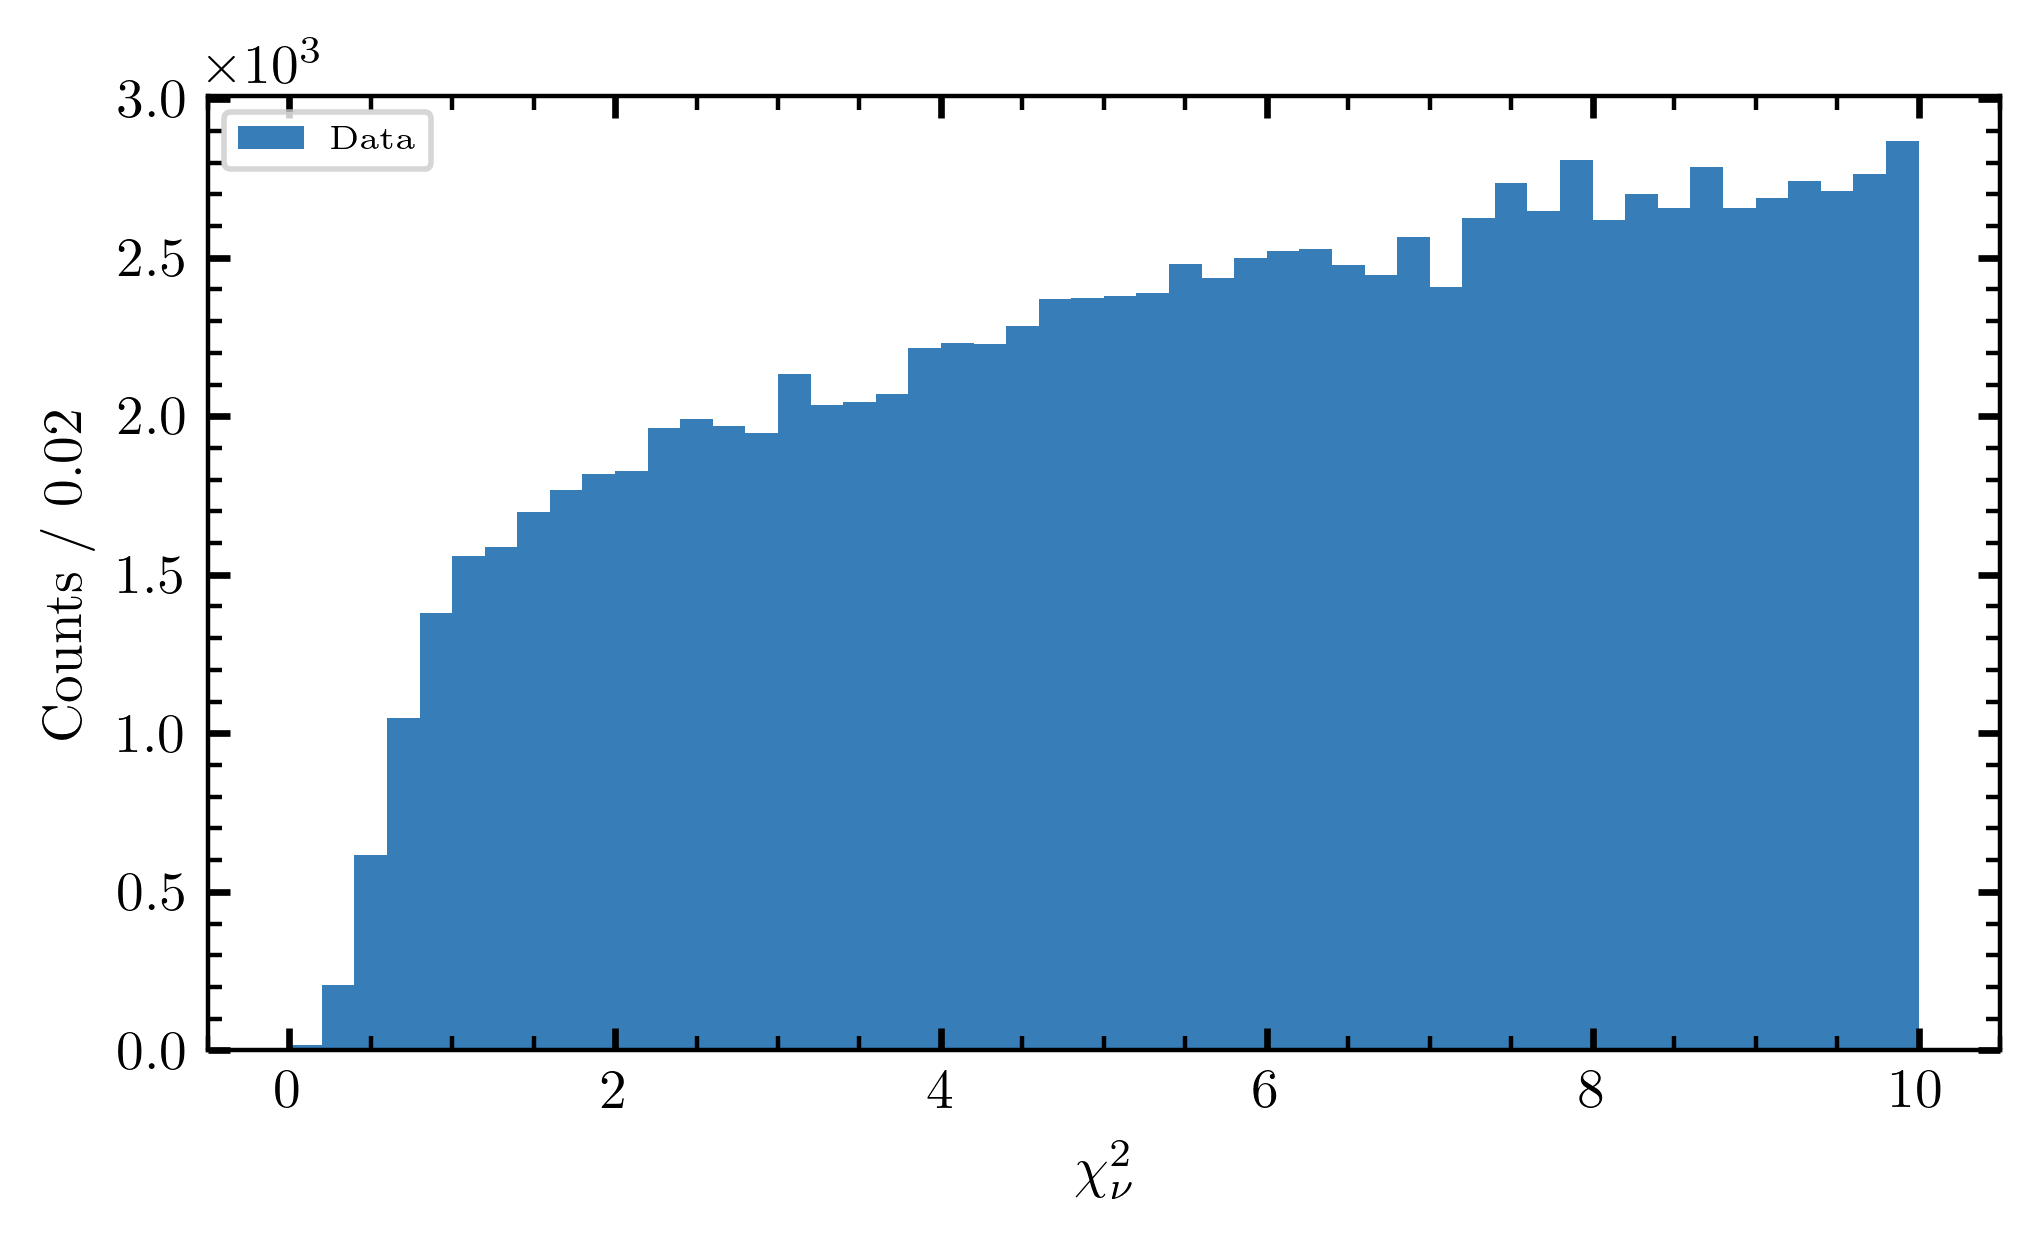
\includegraphics[width=1\linewidth]{figures/chisqdof_data_accpol.png}
      \caption{}
      \label{fig:chisqdof-data}
    \end{subfigure}
    \begin{subfigure}[b]{.8\columnwidth}
      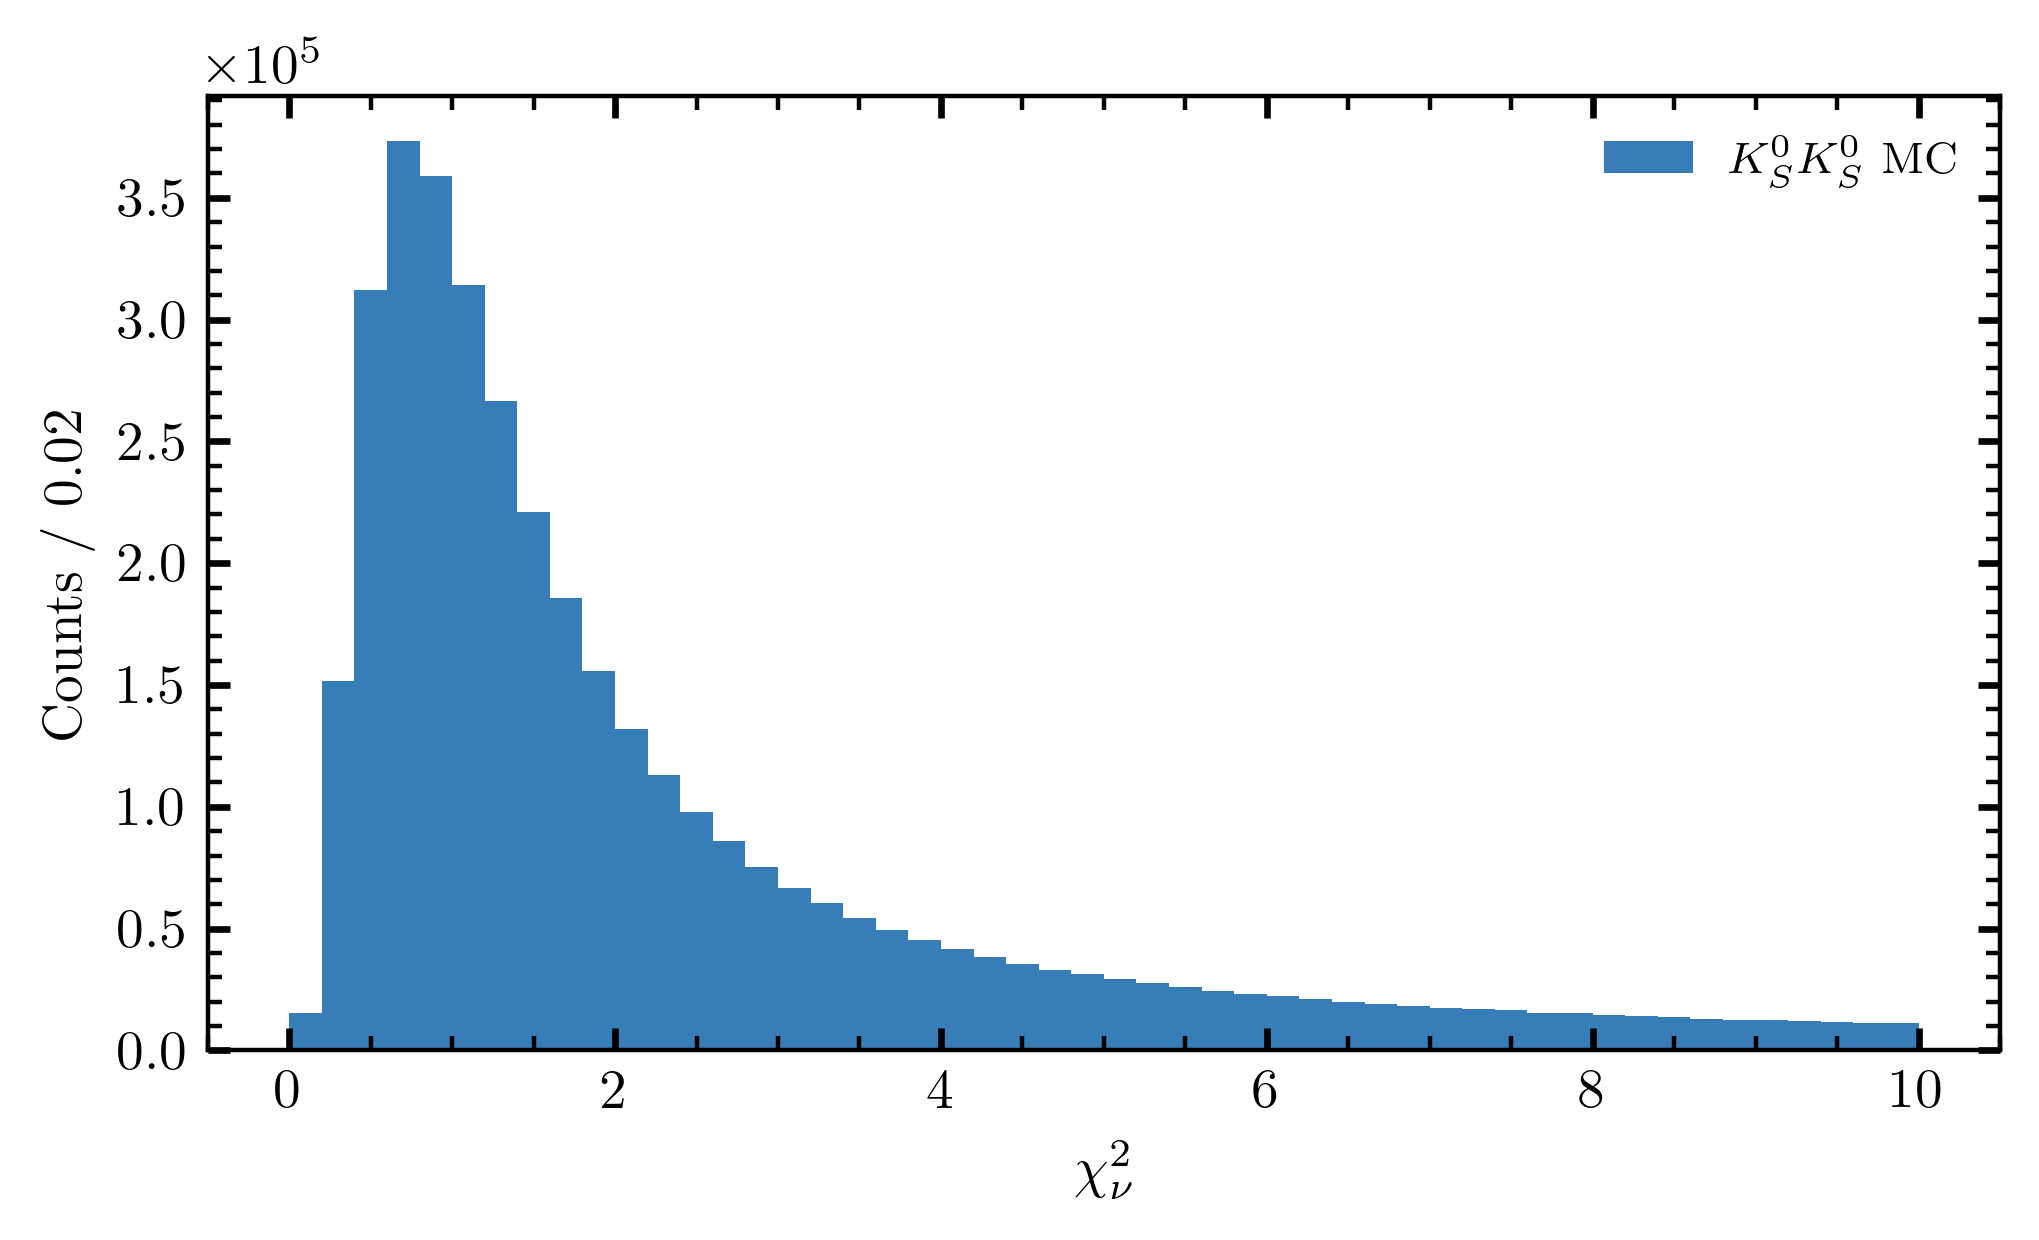
\includegraphics[width=1\linewidth]{figures/chisqdof_accmc_accpol.png}
      \caption{}
      \label{fig:chisqdof-mc}
    \end{subfigure}
  \end{center}
  \caption{Distributions of $\chi^2_\nu$ (the $\chi^2$ per degree of freedom of the GlueX kinematic fit) for (a) data and (b) signal Monte Carlo after reconstruction cuts but before any fiducial selections from \Cref{sub:fiducial-cuts}. Note that the data extends past $\chi^2_\nu > 10$, but the plot was truncated for legibility. Both datasets have had accidental subtraction applied and combos flattened (see \Cref{subsub:combos,sec:data-selection}).}\label{fig:chisqdof-initial}
\end{figure}


The constraints $\vec{f}$ used in this channel include four-momentum conservation,

\begin{equation}
  \sum_{f\in\text{final}} p^\mu_{f} - \sum_{i\in\text{initial}} p^\mu_{i} = 0^\mu
\end{equation}

where the sum over four-momenta of of the initial-state particles must match that of the final-state particles, and the masses of each intermediate $K_S^0$,

\begin{equation}
  p_{K_S^0}^2 - m_{K_S^0}^2 = 0
\end{equation}

where $m_{K_S^0}$ is the known mass of the $K_S^0$ and $p_{K_S^0}$ is the fitted estimate of the four-momentum reconstructed from the $\pi^+\pi^-$ four-momentum measured by the detectors. Additionally we constrain the initial and final positional vertices of each production step in the topology. For this channel, this means we constrain the initial production vertex and the point of closest approach of the $K_S^0$s and recoil proton, as well as the decay vertex of each $K_S^0$ with the closest approach of its constituent pions. It is important to note that this vertex constraint cannot be done in the case where a $K_S^0$ decays to $2\pi^0$, since the neutral pions will decay to $2\gamma$ which can only be detected the calorimeters. Because there is not a second point of detection for these photons, their trajectory and therefore the point at which the original $\pi^0$ decayed is unknown, so there is no way to further reconstruct the kaon decay vertex because the point of closest approach is unknown\footnote{The best we could do would be to assume the kaon decayed at the initial reaction vertex inside the target, which is not only unrealistic given that kaons decay via the weak interaction, but also causes problems later when we try to calculate the kaon lifetime to use in event weighting in \Cref{sec:splot}.}. Therefore, when we specify channels where one or both kaons decay as $K_S^0\to 2\pi^0$, we do not include these $K_S^0$s in the kinematic fit at all, and must infer them by adding the $\pi^0$ four-momenta (see {\color{red} SECTION}). For the main $\gamma p \to K_S^0K_S^0p \to 2\pi^+2\pi^-p$ channel, we have four constraints from four-momentum conservation, two mass constraints (one for each kaon), 14 vertex constraints (two for each constrained particle, viz. four pions, two kaons, and a proton), and nine unknowns from the vertex constraints (the position of the vertex introduces three unknowns for each vertex, and there are three constrained vertices, viz. two kaon decays and the initial production vertex). This gives a total of 20 constraints with nine unknowns, or 11 degrees of freedom in the fit.

\subsubsection{Combos}\label{subsub:combos}

While the initial interaction vertex in theory contains a single photon, in practice, the incident beam contains multiple tagged photons, any of which might provide the requisite energy needed to kinematically generate a given set of final-state tracks. Additionally, there could be multiple ways to recombine or identify final-state particles to arrive at the same event topology. The GlueX reconstruction process considers all valid combinations of tagged photons and sets of reconstructed final-state particles and saves each one in a sub-event called a ``combo''. Each event has at least one of these combos, and some events may have many due to there being many candidate beam photons with similar energies. Since only one combo can be the true event, we need to flatten the data in a way that avoids double counting events. The method for doing so is discussed in {\color{red} SECTION}.
